\section{Conference Venue}

 \begin{figure}[h!]
  \centering
      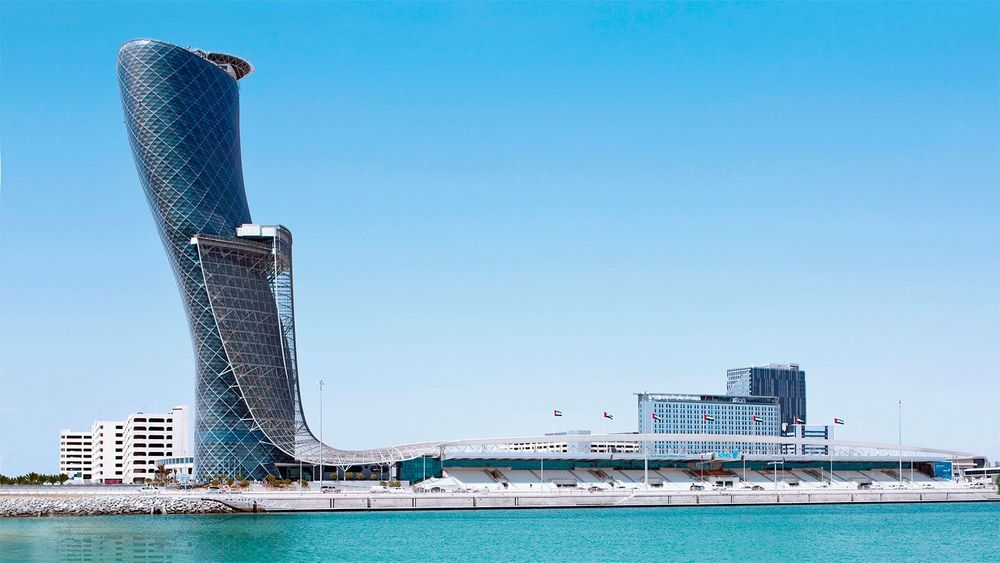
\includegraphics[width=0.9\linewidth]{/Users/uniba/Documents/GitHub/aclpub2/examples/handbook_acl/local_guide/images/location.png}
 \end{figure}

Venue.
\section{About Ireland}

About.
\section{About Dublin}

 \begin{figure}[h!]
  \centering
      \includegraphics[width=0.9\linewidth]{/Users/uniba/Documents/GitHub/aclpub2/examples/handbook_acl/local_guide/images/dublin.png}
 \end{figure}
 \leavevmode\newline

Info. \\

\section{Enjoying Ireland}

 \begin{figure}[h!]
  \centering
      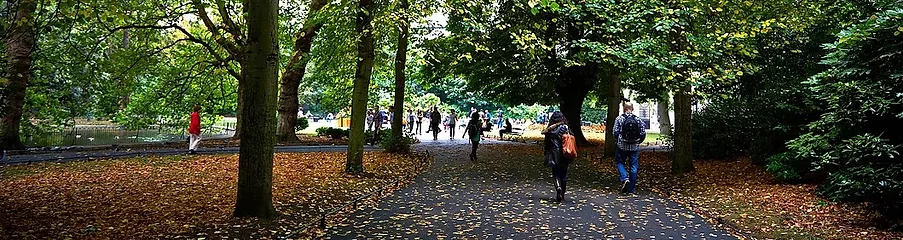
\includegraphics[width=0.9\linewidth]{/Users/uniba/Documents/GitHub/aclpub2/examples/handbook_acl/local_guide/images/green.png}
 \end{figure}
 \leavevmode\newline

{\Large \textit{Top Visitor Attractions}}\\
Attractions. \\


 \leavevmode\newline
\section{important Information}

{\large \textbf{Climate}}\\
Abu Dhabi has a northern-hemisphere subtropical, arid climate. November to March is the most appealing time of year, and it is also when infrequent winter rains occur.
The temperature range in the winter months is between 56 F (13 C) and 75 F (24 C) with typically bright sunny days which correspond to the best kind of spring weather in the US.\\

{\large \textbf{Clothing}}\\
Summer clothing may be worn for most of the year, but during the winter evening temperatures may occasionally call for a jacket or light coat. 
While dress codes are fairly liberal, consideration should be given not to offend the sensibilities of others. 
Swimwear should be worn only on beaches or at swimming pools. Visiting shopping malls and other attractions, tourists should wear clothing that is not too tight or revealing. 
Certain attractions such as mosques or religious sites usually have stricter dress codes, requiring both men and women to cover up bare shoulders, arms and legs, and women to wear headscarves.\\

{\large \textbf{Communications}}\\
The international dialing code for incoming calls to landlines in the UAE is +971 and 02 for Abu Dhabi. 
Calls to and from landlines within Abu Dhabi are free. Direct dialing is possible to over 170 countries. 
UAE has two mobile networks, Du and Etisalat:
\begin{itemize}
    \item Both offer temporary SIM cards for tourists and business travelers, including data and calls, and these can be purchased at outlets across the UAE, including at the airport and malls.
    \item Roaming services are also available for most visitors if they wish to use their existing number and phone.
\end{itemize}

{\large \textbf{Currency and Living Cost}}\\
The monetary unit is the Dirham (AED), which is divided into 100 fils. The exchange rate is pegged to the US Dollar at the rate \$1 = AED 3.675.\\
The average costs at an average coffee shop or restaurant are as follows:
\begin{itemize}
    \item Cup of coffee: 14-20 AED/\$3.8-5.5 USD
    \item Sandwich lunch: 15-30 AED/\$5-8.2 USD
    \item Evening meal: 30-50 AED/\$8.2–13.6 USD
\end{itemize}

{\large \textbf{Electricity}}\\
The electricity supply in Abu Dhabi is 220/240 volts at 50 cycles.
Standard British-type 13-amp square three-pin plugs are the norm in most hotels. 
European or US-made appliances may need a plug adapter.\\

{\large \textbf{Language}}\\
The official language of the UAE is Arabic. However, English is also very widely spoken throughout Abu Dhabi, 
especially in business, hospitality, retail environments, street signs, taxis, restaurant menus, etc.
Urdu and Hindi are also widely spoken.\\
Top eight phrases to learn:
\begin{itemize}
    \item Marhaba مرحبا Hello
    \item Ahlan أهلاً Welcome
    \item Ma’asalama مع السلامة Good Bye
    \item Shukran شكراً Thank you
    \item Mabrook مبروك Congratulations
    \item Yalla يلا Let’s go
    \item Khalas خلص enough/done
    \item Inshallah إن شاء الله God willing, may be, no, and a host of other context dependent meanings.
\end{itemize}

{\large \textbf{Security}}\\
As one of the most cosmopolitan and multicultural cities in the world, home to over 200 different nationalities, 
 Abu Dhabi is an advocate for peace and stability, and proud to be a connecting hub between East and West.
Abu Dhabi is ranked in the 10 safest cities by Aon Hewitt, with low crime rates, a stable government,
 and a department of Abu Dhabi Police dedicated entirely to visitors.\\

{\large \textbf{Taxation}}\\
The UAE does not levy income tax on individuals. Value Added Tax is levied on a majority of goods and services.\\

{\large \textbf{Time Zone & Business Hours}}\\
Abu Dhabi is GMT+4. Most businesses are open from 8 am to 6 pm, Monday to Friday,
 with Saturday and Sunday being official holidays for all government departments. 
Embassies, consulates, and government offices operate from 7:30 am to 2:30 pm, Monday to Friday.\\

{\large \textbf{Tipping}}\\
Tipping practices are similar to most other parts of the world. 
Most restaurants include a 10\% service charge, but tipping, in general, is at the customer’s discretion.\\

{\large \textbf{Water}}\\
The tap water in Abu Dhabi is safe to drink. But locally bottled water is generally served in hotels and restaurants.\\

{\large \textbf{Emergency}\\}
The emergency phone number for Abu Dhabi Police is 999. 
Whether you need police assistance, an ambulance, or for any other emergency, 999 is the number to call and calls are free. 
When calling 999, please remember to state your name, the nature of the accident, address of the emergency and how serious the situation is. 
Please find a detailed list of other emergency numbers at the bottom of this page.

If you’re involved in a traffic accident, it’s important to contact the police immediately. 
In case of a minor incident, move your car to the roadside, as there are fines for obstructing traffic. 
Remember, you cannot file an insurance claim without a police report.

For other enquiries, Abu Dhabi Police operates a dedicated Tourism Police section which will advise and guide you on a range of matters. 
You can contact them on +971 2 800 2626 and +971 2 512 7777, or visit Emergency Help for Tourists.

In a medical emergency, Abu Dhabi’s Sheikh Khalifa Medical City (+971 2 819 0000) and Mediclinic Al Noor Hospital (800 2000) both have Accident and Emergency units. 
If you’re injured in a traffic accident, you will automatically be taken to Sheikh Khalifa Medical City, as it has the best Accident & Emergency treatment facilities.

The Abu Dhabi Government portal provides an updated list of 24-hour pharmacies and medical services, including hospitals, clinics, and medical centres. 
If you don’t have internet access you can call the toll-free number 800 555 (+971 2 666 4442).\\

\section{Visa \& Passport}
Visa.

{\large \textbf{Do I need a visa?}}\\
Please consult with the relevant Irish Embassy/Consulate/Visa Office or visit the official government website: \\
\url{https://www.dfa.ie/travel/visas/visas-for-ireland/}

 \leavevmode\newline


 \leavevmode\newline
\section{Travel to the Conference Venue}

 \begin{figure}[h!]
  \centering
      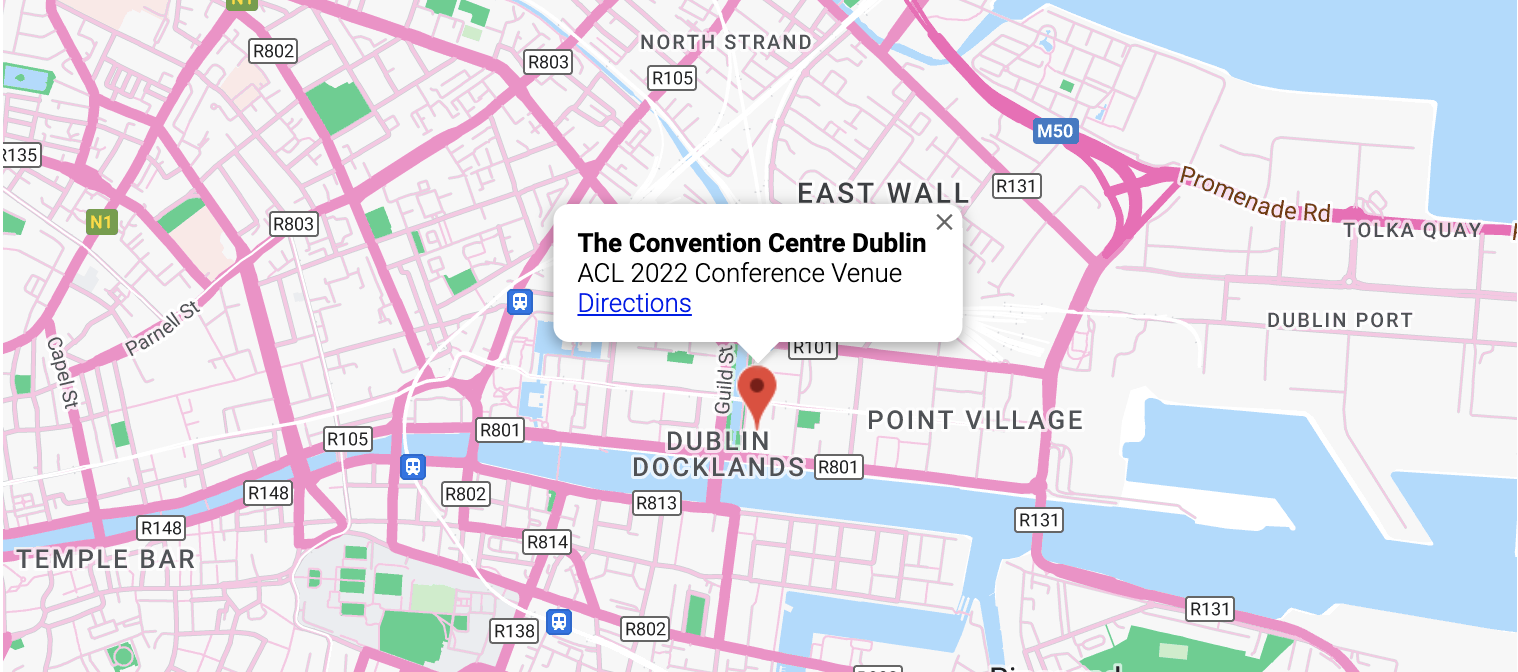
\includegraphics[width=0.9\linewidth]{/Users/uniba/Documents/GitHub/aclpub2/examples/handbook_acl2022/local_guide/images/map.png}
 \end{figure}
 \leavevmode\newline
Travel.